% Figure: incremental fingerprint graph (story 5).
% Build: pdflatex fingerprint_graph.tex  (run inside figures/)
\documentclass[tikz,border=6pt]{standalone}
\usetikzlibrary{positioning,arrows.meta}
\begin{document}
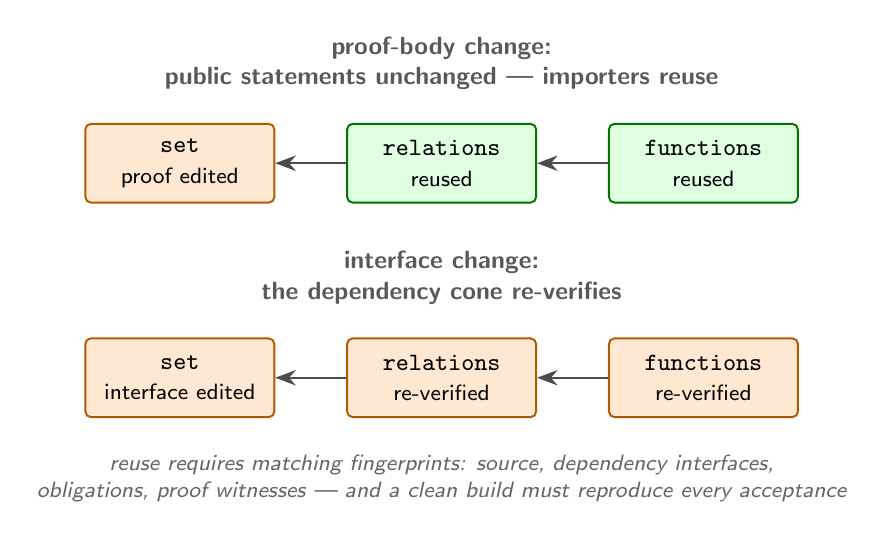
\begin{tikzpicture}[
  font=\sffamily,
  mod/.style={draw, rounded corners=2pt, align=center, minimum width=24mm,
              minimum height=10mm, line width=0.7pt, font=\sffamily\small},
  fresh/.style={mod, fill=blue!10, draw=blue!50!black},
  redo/.style={mod, fill=orange!18, draw=orange!70!black},
  keep/.style={mod, fill=green!12, draw=green!45!black},
  dep/.style={-{Stealth[length=2.6mm]}, line width=0.9pt, black!70},
  plabel/.style={font=\sffamily\small\bfseries, text=black!65, align=center},
  note/.style={font=\sffamily\footnotesize\itshape, text=black!60, align=center},
]
  % Scenario 1: proof-body edit
  \node[redo] (a1) {\texttt{set}\\ \footnotesize proof edited};
  \node[keep, right=9mm of a1] (b1) {\texttt{relations}\\ \footnotesize reused};
  \node[keep, right=9mm of b1] (c1) {\texttt{functions}\\ \footnotesize reused};
  \draw[dep] (b1) -- (a1);
  \draw[dep] (c1) -- (b1);
  \node[plabel, above=3mm of b1]
    {proof-body change:\\ public statements unchanged --- importers reuse};

  % Scenario 2: interface edit
  \node[redo, below=17mm of a1] (a2) {\texttt{set}\\ \footnotesize interface edited};
  \node[redo, right=9mm of a2] (b2) {\texttt{relations}\\ \footnotesize re-verified};
  \node[redo, right=9mm of b2] (c2) {\texttt{functions}\\ \footnotesize re-verified};
  \draw[dep] (b2) -- (a2);
  \draw[dep] (c2) -- (b2);
  \node[plabel, above=3mm of b2]
    {interface change:\\ the dependency cone re-verifies};

  \node[note, below=3.5mm of b2]
    {reuse requires matching fingerprints: source, dependency interfaces,\\
     obligations, proof witnesses --- and a clean build must reproduce
     every acceptance};
\end{tikzpicture}
\end{document}
